\documentclass{acm_proc_article-sp}

\usepackage{graphicx}% Include figure files
\usepackage{caption}
\usepackage{subcaption}
\usepackage{dcolumn}% Align table columns on decimal point
\usepackage{bm}% bold math
\usepackage{amsmath}
\usepackage{float}
\usepackage{array}
\usepackage{verbatim}
\usepackage{tikz}
\usepackage{hyperref}% add hypertext capabilities
\usepackage{xcolor}
%\usepackage[mathlines]{lineno}% Enable numbering of text and display math
%\linenumbers\relax % Commence numbering lines


\usepackage{listings}
%\usepackage{footnote}
%\makesavenoteenv{table}
%\makesavenoteenv{table*}
%\makesavenoteenv{tabular}

\begin{document}

\title{Self-Organizing systems WS14\\
       Hexagonal SOM extension}

\numberofauthors{2}
\author{
Richard Plangger\\
\email{e1025637@student.tuwien.ac.at}
\alignauthor
Rene Koller\\
\email{e0925021@student.tuwien.ac.at}
\alignauthor
}

\date{\today}

\maketitle

\begin{abstract}
    This document describes our solution to the assignment
    to extend the SOM Toolbox to train and display a hexagonal
    SOM
\end{abstract}

\keywords{Self organizing systems, SOM, hexagonal, training}

\section{SOM Toolbox}

For this assignment we used the SOM Toolbox~\cite{somtoolbox}. Our solution
is based on the source code found in the section ``Download Latest'' and is
identified by the version ``0.7.5-4.svn4332''. In the deliverable of this assignment we attached a patch that can be applied to the root folder of the project. It is called ``hexagonal.diff''. The modified source code can also be obtained from the repository located at~\url{https://github.com/planrich/sos-ws-14} and is located in the subfolder ex3.

\section{Terminology}

As shown in Figure~\ref{fig:coord} both hexagonal and rectangular
use the same coordinate system to reference nodes from their memory.
There was no need to modify the array cell layout, but only adjust the
calculation for the grid neighbors. The major
difference while using hexagonal grid system is that there are not only
four direct neighbors but six.

The neighbors using $(X/Y)$ as coordinate indices of $(1/1)$ in Figure~\ref{fig:coord-rect}
are $\{(1/2),(2/1),(1/0),(0/1)\}$. In Figure~\ref{fig:coord-hex} they are $\{(1/2),(2/2),(2/1),(2/0),(1/0),(0/1)\}$.

The hexagonal grid is rendered ``pointy top''\footnote{The hexagon is rotated in such a way that an edge points up} and every second row is shifted half width of a
cell to the left.

\begin{figure}
    \begin{subfigure}{1\linewidth}
    \centering
    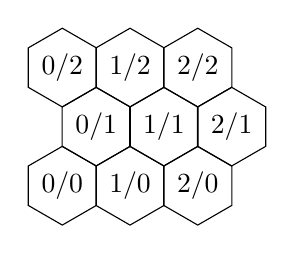
\begin{tikzpicture}
        \foreach \off / \x / \y in {0/0/0,0/1/0,0/2/0,0.43cm/0/1,0.43cm/1/1,0.43cm/2/1,0/0/2,0/1/2,0/2/2} {
            \draw ({\off + \x*0.86cm},{0.75cm * \y}) -- ++(30:0.5cm)
              \foreach \r in {90,150,210,270,330} { -- ++(\r:0.5cm) }
              -- cycle;
          \draw ({\off + \x*0.86cm},{0.75cm * \y + 0.5cm}) node {\x/\y};
        };
    \end{tikzpicture}
    \caption{hexagonal}
    \label{fig:coord-hex}
    \end{subfigure}

    \begin{subfigure}{1\linewidth}
        \centering
    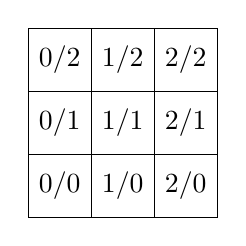
\begin{tikzpicture}
        \foreach \off / \x / \y in {0/0/0,0/1/0,0/2/0,0.43cm/0/1,0.43cm/1/1,0.43cm/2/1,0/0/2,0/1/2,0/2/2} {
            \draw ({0.8cm * \x},{0.8cm * \y})
              -- ++({0.8cm},{0})
              -- ++({0},{0.8cm})
              -- ++({-0.8cm},{0})
              -- cycle;
          \draw ({\x*0.8cm + 0.4cm},{0.8cm * \y + 0.4cm}) node {\x/\y};
        };
    \end{tikzpicture}
    \caption{rectangular}
    \label{fig:coord-rect}
    \end{subfigure}
    \caption{Coordinate system and layout}
    \label{fig:coord}
\end{figure}

To abstract the grid neighborhood, geometric layout and rendering from the actual 3d \lstinline!Unit! array
representation a new interface has been introduced. The interface \lstinline!GridGeometry! is the base abstraction
to be able to calculate shapes, center of the shapes and the grid neighbors.

\section{Hexagonal Training}

By examining the training process implemented in \lstinline!GrowingLayer! we have identified the following two strategies.
First there is the single threaded training calculating the neighborhood using the function presented in the lecture:
\[
    h_{ci} = \alpha \times exp \left(-\frac{dist(winner,unit)^2}{2\sigma^2}\right)
\]
In the function \lstinline!updateUnitsInArea! $h_{ci}$ is the used to updated the weight vectors for each unit.

The second strategy is called batch SOM that, similar to the first strategy, uses the squared distance to the neighbors
to mark the activation. It then updates the weight vector of every node by assigning the mean value of all mapped input
data samples in the neighborhood.

Since the algorithms are so similar we decided not to duplicate the SOM training code contained in \lstinline!GrowingLayer! but
rather just abstract the distance measures. The main advantage of our approach is that all features of the growing layer (such as adding and removing columns for a non static SOM) can now also be used with a hexagonal grid.

Both strategies mentioned earlier solely rely on the distance measure in the grid geometry.
Figure~\ref{fig:hci-coord-rect} illustrates the rectangular distance measurement.
The inner dashed circle has an euclidean distance of $\sqrt{1} = 1$ to
the unit center at position $(1,1)$. The geometry layout in the code does not calculate the distance from the center of
the unit square, but from the corner (lower left). The distance for the second dashed circle has an euclidean distance of $\sqrt{2} \approx 1.14$ and finally the last circle has a distance from the unit (1/1) of $\sqrt{4} = 2$.

To achieve the same distances in a hexagonal grid our approach is visualized in Figure~\ref{fig:hci-coord-hex}.
The inner circle has a distance of $1$ to all of his 6 neighbors. To achieve this distance metric
we use the rectangular unit space which with an distance metric $u$ from any neighboring unit. The hexagon grid forces deformation
of the shapes the following formulas are used to calculate the grid.

\begin{itemize}
    \item Hexagonal width using a reference unit $u$ (e.g cm) is $1$. Trivially
        $ h_w(u) = u; h_w(1) = 1 $
    \item Hexagonal height using a reference unit $u$ \\
        $ h_h(u) = u \times \frac{2}{\sqrt{3}} * \frac{3}{4}; h_h(1) \approx 0.86 $
    \item Hexagonal shift\footnote{Note that the hexagonal shift only returns a non zero
    	value for every second row.} using a reference unit $u$ \\
        \[ h_s(u) = \left\{
               \begin{array} {l l}
                   h_w(u)/2 & \mathrm{if}\ index(row)\mod 2 = 1 \\
                   0 & \mathrm{otherwise}
               \end{array}
               \right.\]

    \item Euclidean distance formula.
    \begin{align*}
        d(p_1,p_2) & = \sqrt{ A^2 + B^2 }\\
        A & = (h_w(1) * p_2.x + h_s(1)) \\
          &- (h_w(1) * p_1.x + h_s(1))\\
        B & = (h_h(1) * p_2.y) - (h_h(1) * p_1.y)
    \end{align*}
    $p_x$ is a point in the rectangular grid. The dot-operator $x$ and $y$
    (e.g. $p_1.x$) get the rectangular position. Thus $d(p_1,p_2)$ is just the
    euclidean distance adjusted by the hexagonal shape width and height
    and every second row shifted by half of the width.
\end{itemize}

\begin{table}
	\centering
	\begin{tabular}{|l|c|c|c|c|}
		\hline
		  & $r=1$& $r=2$ & $r=3$ & $r=4$ \\
		\hline
		Rect. $\mathrm{euclidean}^2$ & 4 & 8 & 8 & 12 \\
		\hline
		Hex. $\mathrm{euclidean}^2$ & 6 & 6 & 12 & 18 \\
		\hline
		\hline
		Rect. $\mathrm{euclidean}$ & 4 & 12 &  28 & 48 \\
		\hline
		Hex. $\mathrm{euclidean}$ & 6 & 18 & 36 & 60 \\
		\hline
	\end{tabular}
	\caption{Neighbouring units using different grid layout and distance measures. Columns show different radius values $r$.}
	\label{tab:neighbours}
\end{table}

Table~\ref{tab:neighbours} shows the amount of neighbors in a $100\times100$ grid. The unit to measure the distance from is located at index $(50,50)$. Notably using the squared euclidean distance it can happen that for a radius of 2 hexagonal grid has less neighbors than the rectangular one. This can also be observed in Figure~\ref{fig:hci-coord-hex} at position $(0,0)$. The squared distance from $(1,1)$ is 3 which is greater than 2. The black solid circle shows a radius of distance 2.
For all others, we have observed and for the subset we added to the table, hexagonal has always more neighbors than the rectangular one.

Figure~\ref{fig:hci-coord-hex} and~\ref{fig:hci-coord-rect} show the activation of neighbors using three dashed circles. Each circle intersects exactly with 6 nodes centers in the hexagonal grid and 4 nodes in the rectangular grid.

\colorlet{c1}{red}
\colorlet{c2}{violet}
\colorlet{c3}{cyan}
\colorlet{c4}{black}

\begin{figure}
    \begin{subfigure}{1\linewidth}
    \centering
    \begin{tikzpicture}
        \foreach \off / \x / \y in {0/0/0,0/1/0,0/2/0,0/3/0,
                         0.43cm/0/1,0.43cm/1/1,0.43cm/2/1,0.43cm/3/1,
                         0/0/2,0/1/2,0/2/2,0/3/2,
                         0.43cm/0/3,0.43cm/1/3,0.43cm/2/3,0.43cm/3/3} {
            \draw ({\off + \x*0.86cm},{0.75cm * \y}) -- ++(30:0.5cm)
              \foreach \r in {90,150,210,270,330} { -- ++(\r:0.5cm) }
              -- cycle;
          \draw ({\off + \x*0.86cm},{0.75cm * \y + 0.5cm}) node {\x/\y};
        };

        \draw [fill,black] ({0.86cm * 1 + 0.43cm},{0.75cm * 1 + 0.5cm}) circle [radius=0.06cm];

        \draw [dashed,c1] ({0.86cm * 1 + 0.43cm},{0.75cm * 1 + 0.5cm}) circle [radius=0.86cm];
        \draw [dashed,c2] ({0.86cm * 1 + 0.43cm},{0.75cm * 1 + 0.5cm}) circle [radius={0.75cm * 2}];
        \draw [dashed,c3] ({0.86cm * 1 + 0.43cm},{0.75cm * 1 + 0.5cm}) circle [radius={2.2821cm}];
        \draw [c4] ({0.86cm * 1 + 0.43cm},{0.75cm * 1 + 0.5cm}) circle [radius={0.86cm * 2}];
        \foreach \off / \x / \y in {0/1/0,0/2/0,0.43cm/0/1,0.43cm/2/1,0/1/2,0/2/2} {
            \draw [fill,c1] ({\off + 0.86cm * \x},{0.75cm * \y + 0.5cm}) circle [radius=0.06cm];
        };
        \foreach \off / \x / \y in {0/0/0,0/0/2,0/3/2,0/3/0,0.43cm/1/3} {
            \draw [fill, c2] ({\off + 0.86cm * \x},{0.75cm * \y + 0.5cm}) circle [radius=0.06cm];
        };
        \draw [fill,c3] ({0.43cm + 0.86cm * 3},{0.75cm * 3 + 0.5cm}) circle [radius=0.06cm];
    \end{tikzpicture}
    \caption{hexagonal}
    \label{fig:hci-coord-hex}
    \end{subfigure}

    \begin{subfigure}{1\linewidth}
        \centering
    \begin{tikzpicture}
        \foreach \off / \x / \y in {0/0/0,0/1/0,0/2/0,0.43cm/0/1,0.43cm/1/1,0.43cm/2/1,0/0/2,0/1/2,0/2/2} {
            \draw ({0.8cm * \x},{0.8cm * \y})
              -- ++({0.8cm},{0})
              -- ++({0},{0.8cm})
              -- ++({-0.8cm},{0})
              -- cycle;
          \draw ({\x*0.8cm + 0.4cm},{0.8cm * \y + 0.4cm}) node {\x/\y};
        };

        \draw [dashed,c1] ({0.8cm * 1},{0.8cm * 1}) circle [radius=0.8cm];
        \draw [fill,c1] ({0.8cm * 1},{0.8cm * 0}) circle [radius=0.06cm];
        \draw [fill,c1] ({0.8cm * 0},{0.8cm * 1}) circle [radius=0.06cm];
        \draw [fill,c1] ({0.8cm * 2},{0.8cm * 1}) circle [radius=0.06cm];
        \draw [fill,c1] ({0.8cm * 1},{0.8cm * 2}) circle [radius=0.06cm];

        \draw [fill,black] ({0.8cm * 1},{0.8cm * 1}) circle [radius=0.06cm];

        \draw [dashed,c2] ({0.8cm * 1},{0.8cm * 1}) circle [radius={1.1313cm}];
        \foreach \x / \y in {0/0,2/0,2/2,0/2} {
            \draw [fill,c2] ({0.8cm * \x},{0.8cm * \y}) circle [radius=0.06cm];
        }

        \draw [dashed,c3] ({0.8cm * 1},{0.8cm * 1}) circle [radius={0.8cm * 2}];
        \foreach \x / \y in {3/1,1/3} {
            \draw [fill,c3] ({0.8cm * \x},{0.8cm * \y}) circle [radius=0.06cm];
        }
    \end{tikzpicture}
    \caption{rectangular}
    \label{fig:hci-coord-rect}
    \end{subfigure}
    \caption{Coordinate system and layout}
    \label{fig:coord}
\end{figure}

\section{Visualisation}

We have picked two data sets that we will compare in the Sections~\ref{sec:chain-link} and~\ref{sec:chain-iris}. In the following we compiled a list of visualizations that we modified to work for both grid systems.

\begin{itemize}
	\item Activity Histogram
	\item Hit Histogram
	\item U-Matrix
	\item D-Matrix
	\item P-Matrix
	\item Neighbourhood Graph radius
	\item Neighbourhood Graph KNN (K-nearest neighbour)

	\item Quantization Error
	\item Mean Quantization Error
	\item Topographic Error (4/8 units)
\end{itemize}

In every figure we show the rectangular SOM on the left and the hexagonal on the right hand side.
If not noted otherwise the default settings of the visualization is used.

\newcommand{\cmprecthex}[5]
{
	\begin{figure}
		\begin{subfigure}{0.49\linewidth}
			\includegraphics*[width=\linewidth]{img/#1-#2}
			\caption{#5}
			\label{fig:#1-#2-rect}
		\end{subfigure}
		\begin{subfigure}{0.49\linewidth}
			\includegraphics[width=\linewidth]{img/#1-#2-hex}
			\caption{#4}
			\label{fig:#1-#2-hex}
		\end{subfigure}
		\caption{#3}
		\label{fig:#1-#2}
	\end{figure}
}


\subsection{Chain Link}
\label{sec:chain-link}

The chain link dataset describes three dimensional points of two rings that are chained together. Training settings are for both as follows:
\begin{itemize}
	\item Size $x = 12, y = 18$
	\item Learnrate $\alpha = 0.7$
	\item Neighbourhood radius $\sigma = 7$
	\item Iteration count $i = 10000$
\end{itemize}

At a first glance all visualizations produce a very similar result. This is a good sign and indicates that we did preserve the semantics of the training algorithm.

\cmprecthex{cl}{hit}{Hit Histogram}{Hexagonal}{Rectangular}
\cmprecthex{cl}{activity}{Activity histogram. Default referent unit}{Hexagonal}{Rectangular}

By observing Figure~\ref{fig:cl-hit} and~\ref{fig:cl-activity} especially at the latter the
bottom units have different amounts of input data mapped to it. There seems to be one topology
violation in the mid right of both grids. The hexagonal unit (mid right) with 25 units mapped to it has a blue
color. The same is true for the rectangular unit but the topology violation is mapped to two units
having 13 and 15 input mapped to it in Figure~\ref{fig:cl-activity-rect}.

There are 72 interpolating units on the rectangular grid whereas hexagonal has 76 counted in Figure~\ref{fig:cl-hit}. The major difference between the two Hit histograms are that in the
hexagonal case there are more cases where units have a higher amount of input vectors mapped
to them and the average seems to have a more balanced input vector count. These cases occur mostly
on the mid right and left below and above the interpolating units.

\cmprecthex{cl}{dmatrix}{D-Matrix}{Hexagonal}{Rectangular}
\cmprecthex{cl}{pmatrix}{P-Matrix}{Hexagonal}{Rectangular}
\cmprecthex{cl}{umatrix}{U-Matrix}{Hexagonal}{Rectangular}

In both cases of P-Matrix~\ref{fig:cl-pmatrix} and D-Matrix~\ref{fig:cl-pmatrix} there is no notable difference we are aware of.

For the U-Matrix visualization in Figure~\ref{fig:cl-umatrix-hex} we did not interpolate the colors
of the edges of the hexagons that do not have a neighbor. This is done in the rectangular case. Interestingly the hexagonal SOM seems to have more broader mountain regions. The red/orange/yellow line that forms the digit ``2'' or the letter ``Z'' have a stronger orange color meaning that there are higher values in the neighborhood. This could give the impression that coherent regions are better separated in the hexagonal case.

\cmprecthex{cl}{nh-knn-1}{Neighbourhood KNN 1}{Hexagonal}{Rectangular}
\cmprecthex{cl}{nh-knn-2}{Neighbourhood KNN 2}{Hexagonal}{Rectangular}
\cmprecthex{cl}{nh-knn-3}{Neighbourhood KNN 3}{Hexagonal}{Rectangular}
\cmprecthex{cl}{nh-radius-0,1}{Neighbourhood Graph Radius 0.1}{Hexagonal}{Rectangular}
\cmprecthex{cl}{nh-radius-0,2}{Neighbourhood Graph Radius 0.2}{Hexagonal}{Rectangular}
\cmprecthex{cl}{nh-radius-0,3}{Neighbourhood Graph Radius 0.3}{Hexagonal}{Rectangular}

Figure~\ref{fig:cl-nh-knn-1},\ref{fig:cl-nh-knn-2} and \ref{fig:cl-nh-knn-3} show the Neighborhood Graph using KNN with different $k$ values. All of them look similar to their hexagonal neighborhood graph. It can be observed that the hexagonal graph has a staggering pattern in the top and the bottom of the map.
This is considered a good sign because the neighbors are aligned good on the hexagonal grid.
Figure~\ref{fig:cl-nh-knn-3} and the neighborhood graph using a radius in Figure~\ref{fig:cl-nh-radius-0,1} look very similar.  It was mentioned earlier that there is a unit with 25 input samples mapped to it. Above it there is a unit with only two. These units are both connected to an unit in the upper center. This forms a triangle that is not present in the rectangular case.

By examining the neighborhood graph with a higher radius in Figure~\ref{fig:cl-nh-radius-0,2} and~\ref{fig:cl-nh-radius-0,3} the hexagonal unit have more red lines that connect neighbors than the rectangular ones.

\cmprecthex{cl}{qe}{Quantization Error (QE)}{Hexagonal}{Rectangular}
\cmprecthex{cl}{mqe}{Mean Quantization Error (MQE)}{Hexagonal}{Rectangular}

The QE shown in Figure~\ref{fig:cl-qe} does not differ very much comparing the two grid layouts.
But the MQE shown in Figure~\ref{fig:cl-mqe} has much higher values in the hexagonal grid system. Earlier it was already observed that there is a more balanced distribution of unit to mapped input vectors in the hexagonal case. This might be one the reason for the result shown in~\ref{fig:cl-mqe}. The other explanation we could think of is that in the hexagonal case more neighbors are pulled in the training phase. This keeps unit regions until the fine tuning of the map closer together leading to a higher distance to some input samples.

\cmprecthex{cl}{topo-4}{Topographic Error 4}{Hexagonal}{Rectangular}
\cmprecthex{cl}{dist}{Distortion $\sqrt{2}$}{Hexagonal}{Rectangular}

The topographic error in Figure~\ref{fig:cl-topo-4} seems worse in the hexagonal case. Figure~\ref{fig:cl-dist} shows the distortion that is constrainted only to two areas in the hexagonal case.

\subsection{Iris}
\label{sec:iris}

The Iris flower data set or Fisher's Iris data set is a multivariate data set introduced by Sir Ronald Fisher (1936) as an example of discriminant analysis.
The data set consists of 50 samples from each of three species of Iris (Iris setosa, Iris virginica and Iris versicolor). Four features were measured from each sample: the length and the width of the sepals and petals, in centimetres.

Training settings are for both as follows:
\begin{itemize}
  \item Size $x = 10, y = 10$
  \item Learnrate $\alpha = 0.7$
  \item Iteration count $i = 10000$
\end{itemize}

\cmprecthex{iris}{hit}{Hit Histogram}{Hexagonal}{Rectangular}
\cmprecthex{iris}{activity}{Activity histogram. Default referent unit}{Hexagonal}{Rectangular}

Looking at Figure~\ref{fig:iris-hit} and~\ref{fig:iris-activity} we can see that the overall pattern is nearly identical.
Upon closer inspection we can see that in the lower left region the units in Figure~\ref{fig:iris-activity-rect} with more data mapped to it
got more evenly spread out in Figure~\ref{fig:iris-activity-hex}. The top left corner on the other hand shows exactly inverse behaviour where the input data
is more compact and pushed to the edge in Figure~\ref{fig:iris-activity-hex}.

Generally the hexagonal map seems more evenly distributed, even though it also has the unit with the the highest number of input data mapped to it.

\cmprecthex{iris}{dmatrix}{D-Matrix}{Hexagonal}{Rectangular}
\cmprecthex{iris}{pmatrix}{P-Matrix}{Hexagonal}{Rectangular}
\cmprecthex{iris}{umatrix}{U-Matrix}{Hexagonal}{Rectangular}

While the P-Matrix in Figure~\ref{fig:iris-pmatrix} shows no notable differences the hexagonal D-Matrix in Figure~\ref{fig:iris-dmatrix-hex} differs quit a bit from the rectangular on in Figure~\ref{fig:iris-dmatrix-rect}. The first difference can be found in the shape of the colored region, they both start at the same x-position on the top border but the region in the rectangular map curves to the bottom left corner while the region in the hexagonal map stays straight.
The hexagonal Map shows a more defined cluster boundary, most noticable in the center of the mountain region where only the rectengular map has a lower mountain hight.

The U-Matrix for the Iris dataset in Figure~\ref{fig:iris-umatrix} shows the same differences as the U-Matrix for the Chainlink dataset in Figure~\ref{fig:cl-umatrix}, with a broader more well defined mountain region.

\cmprecthex{iris}{nh-knn-1}{Neighbourhood KNN 1}{Hexagonal}{Rectangular}
\cmprecthex{iris}{nh-knn-2}{Neighbourhood KNN 2}{Hexagonal}{Rectangular}
\cmprecthex{iris}{nh-knn-3}{Neighbourhood KNN 3}{Hexagonal}{Rectangular}
\cmprecthex{iris}{nh-radius-0,1}{Neighbourhood Graph Radius 0.1}{Hexagonal}{Rectangular}
\cmprecthex{iris}{nh-radius-0,2}{Neighbourhood Graph Radius 0.2}{Hexagonal}{Rectangular}
\cmprecthex{iris}{nh-radius-0,3}{Neighbourhood Graph Radius 0.3}{Hexagonal}{Rectangular}

Figures~\ref{fig:iris-nh-knn-1},~\ref{fig:iris-nh-knn-2} and ~\ref{fig:iris-nh-knn-3} show the Neighborhood Graph using KNN with different $k$ values. All hexagonal maps look very similar to their rectangular counterparts.
While Figures~\ref{fig:iris-nh-radius-0,1} and~\ref{fig:iris-nh-radius-0,2} show less red lines for the hexagonal grid, the inverse is true for Figure~\ref{fig:iris-nh-radius-0,3} where the hexagonal map shows more, tightly connected red lines.

\cmprecthex{iris}{qe}{Quantization Error (QE)}{Hexagonal}{Rectangular}
\cmprecthex{iris}{mqe}{Mean Quantization Error (MQE)}{Hexagonal}{Rectangular}

The QE shonw in Figure~\ref{fig:iris-qe} and the MQE shown in Figure~\ref{fig:iris-mqe} do not differ greatly between the two grid layouts.


\cmprecthex{iris}{topo-4}{Topographic Error 4}{Hexagonal}{Rectangular}
\cmprecthex{iris}{dist}{Distortion $\sqrt{2}$}{Hexagonal}{Rectangular}

The topographic error shown in Figure~\ref{fig:iris-topo-4} seems worse on the edges, especially on the bottom right, for the hexagonal map but better in the center of the map when compared to the rectangular map.
Figure~\ref{fig:iris-dist} shows that the distorion is reduced in the hexagonal case.

\section{Conclusion}

For this last assignment of the lecture Self-Orgainzing Systems we have implemented a hexagonal grid that can be used to train SOM maps. Our implementation is tightly integraded into the current SOM training mechanisms.
In addition to that we have updated many different visualizations to work correctly with the hexagonal grid and compared them using 2 well known datasets (Iris and Chainlink).
Whether or not a hexagonal SOM is superior to a rectangular cannot be answered. We have observed several positive effects such as slightly better cluster separation in the UMatrix. In contrast to that we \textbf{once} observed that the mean quantization error was much higher in the hexagonal case.
In many cases this might just be a question of aesthetics whether one grid looks better than the other.

\bibliography{ref}
\bibliographystyle{plain}

\end{document}
